%+-------------------------------------------------------
%| CGAL Manual : arr.tex
%|
%| Soon to be split into User and Reference Manuals
%+--------------------------------------------------------
%| update log
%|
%| 21 Jun 2000  - Shai Hirsch
%|    arr_ref.tex was cut into an independent file.
%|
%| 04 May 2000  - Shai Hirsch
%|    Splitting into user and reference manual parts. Using new cc macros.
%|
%| 31 Mar 2000  - Shai Hirsch, 
%|    Changes for the 31/3/2000 deadline (differing user and ref.)
%|
%| Version  1.0 - Iddo Hanniel
%|    
%--------------------------------------------------------

%\documentclass[12pt]{book}
%\usepackage{graphics, amssymb,epsfig}
%\usepackage{cprog,cc_manual}

%\def\Ipe#1{\def\IPEfile{#1}\input{#1}}

%\setlength{\evensidemargin}{.0in}
%\setlength{\oddsidemargin}{-0.3in}
%\setlength{\textwidth}{6.8in}
%\setlength{\textheight}{8in}

%\renewcommand{\Re}{{\rm I\!\hspace{-0.025em} R}}
%\newcommand{\normal}[1]{\eta_{#1}}
%\newtheorem{theorem}{Theorem}[section] % section
%\newtheorem{remark}[theorem]{Remark}
%\newtheorem{lemma}[theorem]{Lemma}
%\newenvironment{dfn}{{\vspace*{1ex} \noindent \bf Definition }}{\vspace*{1ex}}
%\newcommand{\bigdef}[2]{\index{#1}\begin{dfn} {\rm #2} \end{dfn}}
%\newenvironment{proof}{{\em Proof:}}{\hfill{\hfill\rule{2mm}{2mm}}}

%\newcommand{\comment}[1]{{\sf * #1 *}}
%\newcommand{\ncomment}[1]{\noindent {\sf * #1 * }}

%\newtheorem{defn}[theorem]{Definition}
%\newcommand{\intsupplanes}{P} 
%\def\C{{\cal C}}
%\def\G{{\cal G}}
%\def\F{{\cal F}}
%\def\I{{\cal I}}
%\def\U{{\cal U}}
%\def\M{{\cal M}}
%\def\eps{{\varepsilon}}
%\def\bd{{\partial}}
%\def\dm{{\cal D}}

% Title
%\title{CGAL Arrangement Specifications}

%\date{ \today }

%\begin{document}

%\tableofcontents

%\maketitle
\chapter{2D Arrangements} \label{I1_ChapterArrangement_2}

\section{Introduction}

\paragraph{2D Arrangement:} Given a collection $C$ of (possibly
intersecting and not necessarily $x$-monotone) curves in the plane,
we construct a collection 
$C''$ in two steps: First we decompose each curve in $C$ into maximal
$x$-monotone curves, thus obtaining the collection $C'$. We then
decompose each curve in $C'$ into maximal connected pieces not
intersecting any other curve in $C'$. This way we obtain the
collection $C''$ of $x$-monotone, pairwise interior disjoint curves.
The {\em arrangement} of the curves in $C$ is the
{\it planar map}(see Chapter~\ref{I1_ChapterPlanarMap})
induced by the curves in $C''$.
 
\paragraph{Curve Hierarchy Tree:} When constructing an arrangement
we decompose each curve $c$ in two steps obtaining the collections $c'$
and $c''$. We regard these collections as levels in a hierarchy of 
curves where the union of the subcurves in each level is the original curve
$c$. We store these collections in a special structure --- a {\em hierarchy
tree}. This structure usually consists of three levels, although
in some cases they can consist of less (e.g., when inserting an $x$-monotone 
curve) or more (when the users define their own {\em split functions} see
Section~\ref{ssec:example4}). The levels are:
\begin{itemize}
\item Curve node level: the root of the tree --- holds the original curve.
\item Subcurve node level: inner nodes of the tree --- hold decomposed
subcurves of
the original curve. In the default mode these are $x$-monotone curves.
\item Edge node level: leaves of the tree --- hold the curves corresponding to
the edges of the planar map induced by the arrangement. These nodes will
be built only in {\em update mode} (by default the arrangement is in
update mode).
\end{itemize}

Figure~\ref{fig:hierarchy} shows an example of a simple arrangement and its 
corresponding curve hierarchy.

%\vspace{-0.3cm}

\begin{figure}
\begin{ccTexOnly}
{\centering \resizebox*{0.8\textwidth}{0.6\textheight}%
{\includegraphics{arr3.eps}}}
\end{ccTexOnly}
\caption{A simple arrangement of two polylines, and its corresponding
hierarchy tree (the edges of the arrangement are numbered according to
their order in the tree).\label{fig:hierarchy}}
\begin{ccHtmlOnly}
<P>
<center><img border=0 src="./arr3.gif" alt=" ">
<!--
<br>
A simple arrangement of two polylines, and its corresponding hierarchy tree
(the edges of the arrangement are numbered according to their order
in the tree).
-->
</center>
\end{ccHtmlOnly}
\end{figure}


The hierarchy tree enables us to intersect the curves without loss of
information. The original curve and the intermediate subcurves are stored
in the tree and the user can traverse them. Furthermore, the users can
define their own hierarchy by passing their own intersection sequence.
This can be of use in some applications. For example, in an arrangement
of spline curves the users might want to intersect a curve in the
junction points before making the curve $x$-monotone. 

\paragraph{Update Mode:} For some algorithms, it is not needed to build
the whole planar map induced by the arrangement. For example, the lower
envelope of an arrangement of $x$-monotone curves which intersect
each other at most a fixed constant $s$ times,
can be found in near linear time \cite{sa-dsstg-95, h-a-97}
even if
the complexity of the planar map induced by it is quadratic.
Therefore, building the planar map induced by the arrangement is not
always desired. The users can therefore disable (or postpone) the building
of the planar map. This is done by disabling the {\it update mode}
using the \ccc{set_update(bool)} member function. When update mode is
set to \ccc{true}, the planar map is updated --- this is the
default situation. 
When update mode is set to \ccc{false}, the hierarchy tree is built without
its \ccc{Edge_level}, and the curves are not inserted into the planar map.

\paragraph{Degeneracies} Like the planar map package (see
Chapter~\ref{I1_ChapterPlanarMap}), the arrangement package can deal with
$x$-degenerate input (including vertical segments). However, while in the
planar map the input curves were assumed to be $x$-monotone and non
intersecting in their interiors, there are no such assumptions in the
arrangement. A non $x$-monotone curve is partitioned into $x$-monotone
subcurves, and curves are intersected in their points of intersection
with other points
before they are inserted into the map. Furthermore, overlapping curves are
supported. If two curves overlap the traits intersection function returns
the two endpoints of the common part. The \ccc{Overlap_circulator}
enables to traverse all overlapping \ccc{edge_nodes} that correspond to
the same pair of halfedges in the map.



%******************************************************************************



\section{Example Programs}
%---------------------------------------------------
\subsection{Simple Example of a Segment Arrangement}
The following example demonstrates the construction of an
$X$-shaped arrangement out of two segments.
After the construction we
traverse the edges of the arrangement in the order defined
by the original segments.

\ccIncludeExampleCode{Arrangement_2/example1.C}

The output of the program looks like this:
\begin{verbatim}
Curve level:
0 0 1 1
Edge level:
0 0 0.5 0.5
0.5 0.5 1 1

Curve level:
0 1 1 0
Edge level:
0 1 0.5 0.5
0.5 0.5 1 0
\end{verbatim}

\subsection{Example of Overlapping Segments}
\label{ssec:example2}
The following example demonstrates the construction of an
arrangement out of two overlapping segments --- $(0,0)-(2,2)$
and $(1,1)-(3,3)$.
After the insertion of the segments we
traverse the halfedges
of the arrangement and count the overlapping curves.
This is done using the \ccc{overlap_edges()} member function that returns an
\ccc{Overlap_circulator}. With it we can circulate
over all the edge nodes that correspond to the halfedge.

\ccIncludeExampleCode{Arrangement_2/example2.C}

The output of the program looks like this:
\begin{verbatim}
Edge 0 0 1 1 is covered by a single edge.
Edge 1 1 2 2 is covered by 2 edges.
Edge 2 2 3 3 is covered by a single edge.
\end{verbatim}


\subsection{Example of a Circle Arrangement}
\label{ssec:example3}
The following example demonstrates the use of the circle traits.
The arrangement created by this example is depicted in
Figure~\ref{fig:circles}.
For this simple example the built-in double
number type will run correctly, it is {\em not} recommended
in the general case. 
The traits are robust only when used with a
number type that supports exact \ccc{sqrt} operations such as LEDA real number type (requires LEDA to be installed
in order to run). 
\begin{figure}[h]
\begin{ccTexOnly}
{\centering \resizebox*{0.8\textwidth}{0.33\textheight}%
{\includegraphics{circles.eps}}}
\end{ccTexOnly}
\caption{The arrangement generated by the example program.\label{fig:circles}}
\begin{ccHtmlOnly}
<P>
<center><img border=0 src="./circles.gif" alt=" ">
<!-- <br>The arrangement generated by the example program. -->
</center>
\end{ccHtmlOnly}
\end{figure}

\ccIncludeExampleCode{Arrangement_2/example3.C}

\subsection{Example of a Polyline Arrangement}
\label{ssec:example10}
The following example demonstrates the use of the polyline traits.
Observe that a polyline Curve is a container (the default STL in this case).
Note that a polyline point is not necessarily  a vertex of the arrangement 
(that is, of the underlying Planar Map).
An edge of the Planar Map need not be a segment (recall the circle traits 
in the above example). The edges are only required to be x-monotone and pairwise disjoint. However, one might expect the planar map (or rather the edge level of the arrangement) to be made of segments alone. 
In the example below point (150, 50) is not a vertex of the planar map. 
The polyline to which it belongs is an edge of the planar map. In such cases the user can define additional level of hierarchies, as shown in the next example.

For this simple example the built-in double
number type will run correctly, it is {\em not} recommended
in the general case. 
The traits are robust only when used with a
number type such as LEDA real number type (requires LEDA to be installed
in order to run). 

\ccIncludeExampleCode{Arrangement_2/example10.C}

\begin{ccAdvanced}
\subsection{Example of a User-defined Hierarchy}
\label{ssec:example4}

The following example demonstrates the construction of an
arrangement of two segments, using a user-defined
hierarchy.
We use a simple split function that splits a segment in its middle
point. We insert the first segment using the user-defined function
and the second segment with the regular function.

\ccIncludeExampleCode{Arrangement_2/example4.C}

The output of the program looks like this:
\begin{verbatim}
Curve level:
0 0 6 6
Edge level:
0 0 3 3
3 3 4 4
4 4 6 6

Curve level:
0 4 6 4
Edge level:
0 4 4 4
4 4 6 4
\end{verbatim}

\end{ccAdvanced}


\begin{ccAdvanced}

\subsection{Example of a User-defined Hierarchy with Function Objects}
\label{ssec:example5}

The following example demonstrates the use of a function object in
a user-defined hierarchy. We define a base class for the function objects
with a virtual \ccc{operator()}, that the function objects override (this
kind of pattern is sometimes called an \ccc{Action} class
(see for example \cite[Chapter~25.5]{s-cpl-97}). This enables us to
use an inner state in our function as is done in the example.

In the example we define two levels of a hierarchy. The first level
splits the inserted segment in the middle. The second layer splits every
curve of the first layer in a ratio of $1/3 : 2/3$. Therefore, after
an insertion of the segment $(0,0) - (6,6)$
we will have four edges (eight halfedges)
inside the arrangement, corresponding to the segments: $(0,0) - (1,1)$,
$(1,1) - (3,3)$, $(3,3) - (4,4)$ and $(4,4) - (6,6)$.

%\ccIncludeExampleCode{example5.C}
\ccIncludeExampleCode{Arrangement_2/example5.C}

\end{ccAdvanced}


% EOF ------------------------------------------------------------------------80










